% !TEX root = ../cours.tex
\chapter{Calcul des propositions}

Le \og \textit{calcul des propositions} \fg{}, autrement appelé \og \textit{logique propositionnelle} \fg{}, est un système formel à la base de la logique mathématique. Le calcul des propositions nous intéresse pour plusieurs raisons:
\begin{enumerate}
\item
Le système nous permet de formaliser la notion de preuve et de discuter des techniques de preuve.
\item
Le système est à la base de la logique des prédicats et de la théorie des ensembles, dont nous auront besoin pour établir certains résultats liés à la cardinalité des ensembles de langages.
\item
Le problème de \og \textit{satisfiabilité} \fg{} d'une formule propositionnelle est fondamental dans l'étude des problèmes \textit{NP-complets}, concept que nous aborderons dans le cadre de la théorie de la complexité.
\end{enumerate}

Le calcul des propositions a pour objet d'étude des \og \textit{propositions} \fg{}.
Une proposition est un fait qui peut être vrai ou faux.
Les propositions sont formées de propositions atomiques (variables et constantes) combinées entre elles par des \og \textit{connecteurs} \fg{} (\textit{et}, \textit{ou}, \textit{seulement si}, etc.).

\paragraph{Exemple}

Pour ce premier exemple, on considère trois variables $p$, $d$ et $m$.
On donne à la variable $p$ la signification \og il pleut \fg{}, à la variable $d$ le sens \og le chat est dehors \fg{} et à la variable $m$ le sens \og le chat est mouillé \fg{}.

Ces variables peuvent être combinées à l'aide de différents connecteurs afin d'exprimer des propositions plus complexes.
Par exemple, alors que la proposition $m$ indique que le chat est mouillé, la proposition $\neg m$ indique que le chat n'est pas mouillé.
La proposition $m \iff p \wedge d$ a pour sens \og le chat est mouillé si et seulement si il pleut et le chat est dehors. \fg{}.
Bien que cette dernière proposition semble intuitivement vraie (étant donné notre interprétation de la réalité), elle n'est pas toujours vérifiée.
Par exemple, si le chat est dehors, qu'il pleut et que le chat n'est pas mouillé, alors la formule sera considérée comme fausse.
Comme on le découvrira par la suite, cette formule n'est pas \og \textit{valide} \fg{}: il existe au moins une interprétation qui rende la formule fausse.

A contrario, si on admet comme hypothèse le fait qu'un chat est mouillé si et seulement si il pleut et que le chat est dehors, et que l'on admette en plus le fait que le chat est mouillé, alors on pourra logiquement en conclure qu'il pleut.
Comme on pourra le montrer, la formule suivante, qui encode ce sens intuitif, est valide.
\[
(m \iff p \wedge d) \wedge m \implies p
\]
Peu importe les valeurs de vérité de $p$, $d$ et $m$, la formule sera toujours vraie.

Nous étudierons aussi un système de preuves formelles, la \og déduction naturelle \fg{}, afin de prouver de manière purement syntaxique de telles propositions.

\section{Syntaxe}

Pour commencer notre étude du calcul des propositions, étudions la \textit{syntaxe} des propositions, c'est-à-dire comment former des propositions (ou \og \textit{formules} \fg{}) bien formées. 

\subsection{Variables propositionnelles}

À la base des formules propositionnelles se trouvent les \og{} \textit{variables propositionnelles} \fg{}.
Chaque variable correspond à une proposition atomique qui peut être vraie ou fausse.
Par convention, on notera les variables propositionnelles avec des lettres minuscules tels que $x$, $y$ ou $z$, ou encore $p$, $d$ et $m$ comme dans l'exemple donné en introduction.

\subsection{Métavariables}

Lors de notre exposition du calcul des propositions, nous ferons aussi appel à des \og \textit{métavariables} \fg{}.
Les métavariables ne font pas partie à proprement parler du langage des propositions: il s'agit simplement d'un moyen de faire référence à des formules arbitraires dans la discussion de la logique propositionnelle.
On utilise des lettres majuscules telles que $A$, $B$ ou $C$ pour dénoter les métavariables.

\paragraph{Exemple} Dans la proposition $A \vee B$, on entend $A$ et $B$ comme des métavariables.
Comme elle contient des métavariables, la proposition $A \vee B$ n'est techniquement pas considérée comme une véritable formule, mais plutôt comme un schéma de formule.
En pratique, cette distinction importe généralement peu, et on parlera aussi de formules pour des schémas de formule.

\subsection{Constantes}

La logique propositionnelle contient deux constantes: \textit{vrai}, que l'on note $\top$ et \textit{faux}, que l'on note $\bot$.
La proposition $\top$ est toujours vraie, alors que la proposition $\bot$ est toujours fausse.

\paragraph{Remarque} Un moyen mnémotechnique pour se souvenir du sens de $\top$ et $\bot$ est de remarquer que $\top$ ressemble à un \texttt{T} comme dans le terme anglais \texttt{True}.

\subsection{Connecteurs}

En logique propositionnelle, on utilise des \textit{connecteurs} afin de composer des formules en formules plus complexes.

\subsubsection{Implication}

On dénote l'implication par une formule $A$ (l'\textit{impliquant}) d'une formule $B$ (l'\textit{impliqué}) par $A \implies B$,
que l'on prononce \og $A$ \textit{implique} $B$ \fg, \og \textit{si} $A$ \textit{alors} $B$ \fg, ou encore \og $A$ \textit{seulement si} $B$ \fg. 

La formule $A \implies B$ est vraie si et seulement si:
\begin{enumerate}
\item
$A$ est fausse, ou,
\item
$B$ est vraie.
\end{enumerate}

Intuitivement, si $A$ est vraie, alors il faut aussi que $B$ soit vraie pour que la formule $A \implies B$ soit vraie.
Dans le cas où l'impliquant $A$ est fausse, alors $A \implies B$ est vraie peu importe la valeur de $B$.
La formule $A \implies B$ ne peut être fausse que si $A$ est vraie et $B$ fausse.

On remarque que $A \implies (B \implies C)$ n'a pas la même signification que $(A \implies B) \implies C$.
On dit que le connecteur ${\implies}$ n'est pas \textit{associatif}.
Pour cette raison, il est important de clarifier ce que l'on entend lorsque l'on utilise plus d'une occurence du connecteur à la suite.
Par convention, on considère que ${\implies}$ associe sur la \textit{droite}.
Par exemple, on considèrera que la formule:
\[
A \implies B \implies C
\]
correspond à la formule:
\[
A \implies (B \implies C)
\]
et non pas à la formule:
\[
(A \implies B) \implies C
\]

\subsubsection{Conjonction}

La \textit{conjunction} de deux formules $A$ et $B$ est notée $A \wedge B$, que l'on prononce \og $A$ \textit{et} $B$ \fg{}.
La formule $A \wedge B$ est vraie si et seulement si $A$ et $B$ sont toutes deux vraies.

Par convention, on considère que le connecteur associe à droite:
\[
A \wedge B \wedge C
\]
correspond à:
\[
A \wedge (B \wedge C)
\]


\subsubsection{Disjonction}

La \textit{disjonction} de deux formules $A$ et $B$ est notée $A \vee B$, que l'on prononce \og $A$ \textit{ou} $B$ \fg{}.
La formule $A \vee B$ est fausse si et seulement si $A$ et $B$ sont toutes deux fausses.
La formule $A \vee B$ est vraie dans tous les autres cas, y compris lorsque $A$ et $B$ sont toutes deux vraies.

Par convention, on considère que le connecteur associe à droite:
\[
A \vee B \vee C
\]
correspond à:
\[
A \vee (B \vee C)
\]

\subsubsection{Négation}

On note la \textit{négation} d'une formule $A$ par $\neg A$, que l'on prononce \og \textit{non} $A$ \fg{}. Contrairement aux autres connecteurs présentés précédemment, on ne considérera pas ce connecteur comme étant \textit{primitif}, mais simplement un raccourci de notation pour exprimer la formule $A \implies \bot$.
\[
\neg A \eqdef A \implies \bot
\]

\subsubsection{Équivalence}

On dénote l'\textit{équivalence} de deux formules $A$ et $B$ par $A \iff B$, que l'on prononce \og $A$ \textit{si et seulement si} $B$ \fg{}. La formule $A \iff B$ est vraie si et seulement si les formules $A$ et $B$ ont la même valeur. Tout comme pour la négation, on ne considérera le connecteur ${\iff}$ que comme un simple raccourci de notation pour dénoter la double implication:
\[
A \iff B \eqdef (A \implies B) \wedge (B \implies A)
\]

On considère que le connecteur associe à droite.
Néanmoins, bien que tout à fait légal, on évitera de former des suites de formules connectées par ${\iff}$.
En effet, la notation:
\[
A \iff B \iff C
\]
pourrait laisser croire que l'on entend que $A$, $B$ et $C$ sont équivalentes, c'est à dire $(A \iff B) \wedge (B \iff C)$,
alors que le véritable sens en est éloigné:
\[
A \iff (B \iff C)
\] 
Ces deux interprétations diffèrent, par exemple lorsque $A$ est vraie et que $B$ et $C$ sont toutes deux fausses.

\subsection{Précédence des opérateurs}

L'usage de parenthèses pour délimiter les sous-formules est parfois verbeux.
Par convention on introduit un ordre de priorité entre les connecteurs afin de simplifier la notation.
On associe à chaque connecteur un niveau de \textit{précédence}. Les connecteurs de plus haute précédence sont appliqués avant ceux de plus basse précédence.

La précédence des connecteurs, par ordre décroissant, est donnée par:
\begin{gather*}
{\neg}\\
{\wedge}\\
{\vee}\\
{\implies}, {\iff}
\end{gather*}
Si bien que la formule:
\[
\neg A \implies B \vee \neg C \wedge D
\]
correspond à la formule:
\[
(\neg A) \implies (B \vee ((\neg C) \wedge D))
\]

\section{Sémantique}

Ayant étudié la syntaxe des propositions, nous pouvons maintenant nous attarder à leur interprétation \og \textit{sémantique} \fg{}, c'est-à-dire à leur sens.

\subsection{Interprétation}

Une \textit{interprétation} $\mathcal{I}$ d'une formule $A$ est une fonction qui associe à chaque variable propositionnelle de $A$ une valeur de vérité: Soit $1$ pour \og vrai \fg, soit $0$ pour \og faux \fg.
La valeur assignée par $\mathcal{I}$ à une variable $x$ est dénotée par $\mathcal{I}(x)$.

On peut aussi dénoter une interprétation sous forme d'ensemble d'associations entre variable et valeur.
Par exemple, $\{ x \mapsto 1, y \mapsto 0 \}$ dénote une interprétation $\mathcal{I}$ qui associe à $x$ la valeur $1$ et à $y$ la valeur $0$. Dans ce cas, on a que $\mathcal{I}(x)$ évalue à $1$ et $\mathcal{I}(y)$ à $0$.

Lorsque $A$ compte $n$ différentes variables propositionnelles, on dénombre $2^n$ interprétations différentes.

\subsection{Évaluation}

Étant donné une interprétation $\mathcal{I}$, une formule $A$ peut être évaluée à $1$ (\og vrai \fg) ou $0$ (\og faux \fg)
en suivant l'interprétation donnés aux variables propositionnelles par $\mathcal{I}$ et
en évaluant les connecteurs en suivant la table de la \cref{fig_tables_connecteurs}.
La constante $\top$ évalue toujours à $1$, alors que la constante $\bot$ évalue toujours à $0$.
On note $A^{\mathcal{I}}$ pour l'évaluation de la formule $A$ par l'interprétation $\mathcal{I}$.

\begin{figure}[h]

\begin{displaymath}
\begin{array}{cc|ccc}
A & B & A \implies B & A \wedge B & A \vee B\\
\hline
1 & 1 & 1 & 1 & 1\\
1 & 0 & 0 & 0 & 1\\
0 & 1 & 1 & 0 & 1\\
0 & 0 & 1 & 0 & 0
\end{array}
\end{displaymath}

\caption{Table de vérité pour les connecteurs primitifs. La table indique le résultat de l'évaluation des formules $A \implies B$, $A \wedge B$ et $A \vee B$ en fonction du résultat de l'évaluation des deux sous-formules $A$ et $B$.}
\label{fig_tables_connecteurs}
\end{figure}

\subsubsection{Modèle d'une formule}

Lorsque une interprétation $\mathcal{I}$ évalue une formule à $1$ (\og vrai \fg), on appelle $\mathcal{I}$ un \textit{modèle} de $A$.
Dans ce cas, on note:
\[
\mathcal{I} \vDash A
\]

Lorsque $A^{\mathcal{I}}$ évalue à $0$ (\og faux \fg), on note:
\[
\mathcal{I} \not\vDash A
\]

\subsubsection{Satisfiabilité}

Une formule $A$ est dite \og \textit{satisfiable} \fg{} s'il existe une interprétation $\mathcal{I}$ tel que $\mathcal{I} \vDash A$.
Une formule $A$ est dite \og \textit{insatisfiable} \fg{} dans le cas ou il n'existe aucun modèle de $A$. 

\subsubsection{Validité}

On dit que $A$ est \og \textit{valide} \fg{} lorsque $A^{\mathcal{I}}$ vaut $1$ pour toutes les interprétations $\mathcal{I}$ possibles – autrement dit, toutes les interprétations sont des modèles.
On dit aussi que la formule est une \og \textit{tautologie} \fg{}.
Dans ce cas, on écrit:
\[
\vDash A
\]

Une formule $A$ est \og \textit{invalide} \fg{} s'il existe une interprétation qui n'est pas un modèle de $A$.

\subsubsection{Relations en validité, invalidité, satisfiabilité et insatisfiabilité}

La~\cref{fig_carre} représente de façon schématique les relations entre les concepts de validité, invalidité, satisfiabilité et insatisfiabilité:
\begin{enumerate}
\item Deux énoncés sont \og \textit{contradictoires} \fg{} si et seulement si quand l'un est faux l'autre et vrai, et inversement. Les concepts de validité et d'invalidité sont contradictoires, ainsi que les concepts de satisfiabilité et insatisfiabilité. Par exemple, une formule est insatisfiable si et seulement si elle n'est pas satisfiable.
\item Deux énoncés sont \og \textit{contraires} \fg{} si et seulement si ils peuvent être simultanément faux mais pas simultanément vrais.
La validité et l'insatisfiabilité sont contraires. Une formule peut être à la fois non valide et non insatisfiable (c'est-à-dire satisfiable), mais une formule ne peut pas être valide et insatisfiable.
\item Deux énoncés sont \og \textit{subcontraires} \fg{} si et seulement si ils peuvent être simultanément vrais mais pas simultanément faux.
L'invalidité et la satisfiabilité sont subcontraires. Une formule peut être à la fois invalide et satisfiable, mais une formule ne peut pas être non invalide (c'est-à-dire valide) et non satisfiable.
\item Deux énoncés sont \og \textit{subalternes} \fg{} si un énoncé implique l'autre. La validité d'une formule implique sa satisfiabité, et l'insatisfiabilité d'une formule implique son invalidité. Validité et satifiabilité sont subalternes, tout comme insatisfiabilité et invalidité.
\end{enumerate}


\begin{figure}[h]
\begin{center}
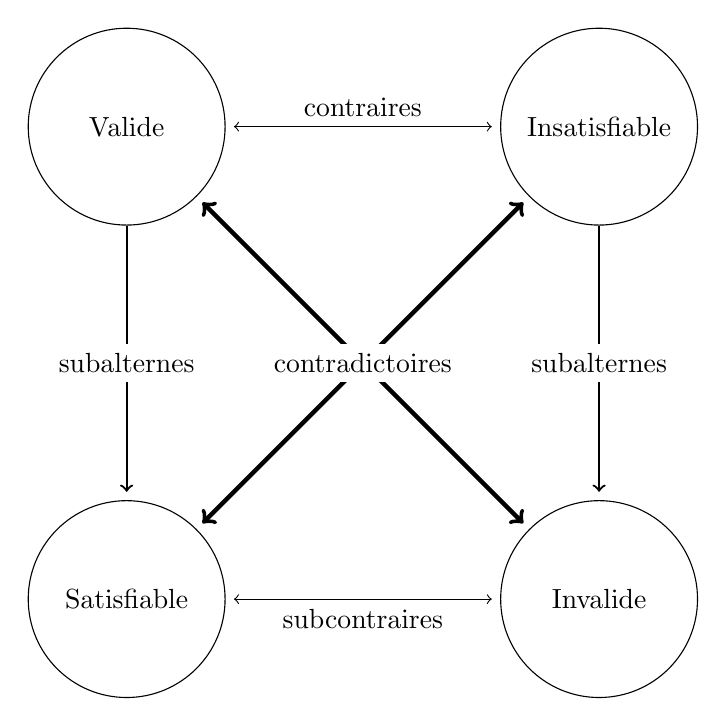
\begin{tikzpicture}
\node[circle, draw, minimum size=2.5cm] (sat) at (2, 2) {Satisfiable};
\node[circle, draw, minimum size=2.5cm] (val) at (2, 8) {Valide};
\node[circle, draw, minimum size=2.5cm] (insat) at (8, 8) {Insatisfiable};
\node[circle, draw, minimum size=2.5cm] (inval) at (8, 2) {Invalide};
\draw[<->, ultra thick, shorten >=3pt, shorten <=3pt] (sat) -- (insat);
\draw[->, thick, shorten >=3pt] (val) -- (sat) node[midway,fill=white] {subalternes};
\draw[<->, shorten >=3pt, shorten <=3pt] (sat) -- (inval) node[below, midway] {subcontraires};
\draw[<->, shorten >=3pt, shorten <=3pt] (insat) -- (val) node[above, midway] {contraires};
\draw[->, thick, shorten >=3pt] (insat) -- (inval) node[midway,fill=white] {subalternes};
\draw[<->, ultra thick, shorten >=3pt, shorten <=3pt] (val) -- (inval);
\node[fill=white] at (5, 5) {contradictoires};
\end{tikzpicture}
\end{center}
\caption{Carré de vérité reliant satisfiabilité et validité.}
\label{fig_carre}
\end{figure}

\subsection{Table de vérité}

Une \og \textit{table de vérité} \fg{} est un tableau indexé par des variables ou métavariables.
Le tableau compte une ligne pour chaque combinaison de valeur de vérité de ces variables.
Les autres colones de la table indiquent le résultat de l'évaluation d'un certain nombre d'autres formules en fonction de la valeur des variables.

Pour les formules complexes, il est parfois plus aisé de rajouter des colonnes pour les sous-formules.

\begin{figure}[h]

\begin{displaymath}
\begin{array}{ccc|ccc}
x & y & z & x \wedge y \vee z & x \vee \neg x & x \iff \neg x\\
\hline
1 & 1 & 1 & 1 & 1 & 0\\
1 & 1 & 0 & 1 & 1 & 0\\
1 & 0 & 1 & 1 & 1 & 0\\
1 & 0 & 0 & 0 & 1 & 0\\
0 & 1 & 1 & 1 & 1 & 0\\
0 & 1 & 0 & 0 & 1 & 0\\
0 & 0 & 1 & 1 & 1 & 0\\
0 & 0 & 0 & 0 & 1 & 0
\end{array}
\end{displaymath}

\caption{Table de vérité indexée par les variables propositionnelles $x$, $y$ et $z$.
Le résultat de l'interprétation des formules $x \wedge y \vee z$, $x \vee \neg x$ et $x \iff \neg x$ en fonction de la valeur des variables $x$, $y$ et $z$ est indiqué dans les trois dernières colonnes.}
\label{fig_table_verite_ex}

\end{figure}

Lorsqu'une colonne ne contient que des $1$, la proposition associée est valide (aussi dit une tautologie).
Si une colonne contient au moins un $1$, alors la proposition associée est satisfiable.
Une colonne qui contient au moins un $0$ indique une proposition invalide.
Finalement, lorsqu'une colonne ne contient que des $0$, la proposition est insatisfiable. 

\paragraph{Exemple} Après examen de la table de vérité de la~\cref{fig_table_verite_ex}, on peut conclure que:
\begin{enumerate}
\item
La formule $x \wedge y \vee z$ est à la fois satisfiable et invalide.
En effet, la formule est satisfiable car il existe un modèle de la formule (par exemple $\{ x \mapsto 0, y \mapsto 1, z \mapsto 1 \}$, à la ligne 5). 
De plus, la formule est invalide car il existe une interprétation qui évalue la formule à $0$ (par exemple $\{ x \mapsto 0, y \mapsto 0, z \mapsto 0 \}$, à la ligne 8).
\item
La formule $x \vee \neg x$ est une tautologie, que l'on note $\vDash x \vee \neg x$. En effet toutes les entrées de la colonne correspondante sont à $1$.
La formule est aussi par conséquent satisfiable.
\item
La formule $x \iff \neg x$ est insatisfiable: toutes les entrées de la colonne correspondante sont à $0$.
La formule est aussi par conséquent invalide.
\end{enumerate}

\section{Déduction naturelle}

La \og \textit{déduction naturelle} \fg{} est un système de preuve pour la logique propositionnelle.
Contrairement à la méthode des tables de vérité, qui est \textit{sémantique}, la \textit{déduction naturelle} est une méthode \textit{syntaxique}.
Il ne s'agit plus d'évaluer des formules, mais de manipuler leur structure syntaxique à l'aide de régles afin d'essayer d'en prouver leur validité.

\subsection{Règle d'inférence}

La déduction naturelle est un système de preuve à base de \og \textit{règles d'inférence} \fg.
Chaque règle est composée d'une \og \textit{conclusion} \fg{}, d'un nombre arbitraire de \og \textit{prémisses} \fg{}, ainsi que d'un nom.

\[
\infer[(\text{nom de la règle})]{\text{conclusion}}{\text{prémisse 1} & \text{prémisse 2} & \dots & \text{prémisse $n$}}
\]

La conclusion et les prémisses d'une règle sont des schémas de formules qui contiennent généralement des métavariables.
Les métavariables qui apparaissent dans la conclusion et les prémisses peuvent être remplacées par n'importe quelle formule, pour autant que ce remplacement se fasse de façon unifiée sur la conclusion et toutes les prémisses dans le schéma.

Intuitivement, une règle d'inférence permet de conclure la conclusion étant donné une preuve de chaque prémisse.

\subsection{Arbre de dérivation}

En déduction naturelle, la preuve formelle d'une formule $A$ prend la forme d'un \og \textit{arbre de dérivation} \fg.
À la racine de l'arbre est une règle d'inférence instanciée avec la formule $A$ pour conclusion.
Chaque prémisse de cette règle doit elle aussi être prouvée, et selon le même procédé.
L'arbre de dérivation a pour feuilles des arbres sans prémisses, que l'on appelle \og \textit{axiomes} \fg{}.
Aussi, comme expliqué plus loin, les feuilles peuvent prendre la forme d'\og \textit{hypothèses déchargées} \fg{}, indiquée par une paire de crochets (\og [ \fg{} et \og ] \fg{}).

\paragraph{Exemple} La~\cref{fig_arbre_derivation} présente un arbre de dérivation pour la formule schématique $A \vee \bot \implies A \wedge \top$. L'arbre de dérivation fait appel à de nombreuses règles d'inférences qui vont être introduites sous peu.

\begin{figure}[h]
\[
\infer[({\Rightarrow{}}I)]{A \vee \bot \implies A \wedge \top}{%
\infer[({\vee}E)]{A \wedge \top}{[A \vee \bot] &%
\infer[({\Rightarrow{}}I)]{A \implies A \wedge \top}{%
\infer[({\wedge{}}I)]{A \wedge \top}{[A] & \infer[({\top}I)]{\top}{}}} &%
\infer[({\Rightarrow{}}I)]{\bot \implies A \wedge \top}{%
\infer[({\bot}E)]{A \wedge \top}{[\bot]}}}}
\]
\caption{Arbre de dérivation de la formule $A \vee \bot \implies A \wedge \top$. L'arbre de dérivation constitue une preuve du théorème $\vdash A \vee \bot \implies A \wedge \top$.}
\label{fig_arbre_derivation}
\end{figure}

\subsection{Théorème}

On appelle un \og \textit{théorème} \fg{} une formule (ou une formule schématique) qui a été prouvée via un arbre de dérivation.
Pour une formule $A$ (ou un schéma de formule), on note $\vdash A$ le fait que $A$ est un théorème.

\subsection{Règles de la déduction naturelle}

Les règles d'inférence de la déduction naturelle sont données ci-après.
Elle sont classifiées en deux catégories: règles d'introduction et règles d'élimination.
Les règles d'introduction introduisent une construction dans leur conclusion,
alors que les règles d'élimination permettent de faire disparaître dans la conclusion une construction apparaissant dans une prémisse.
Les règles sont nommées en fonction de la construction et d'un $I$ ou d'un $E$ suivant s'il s'agit d'une règle d'introduction ou d'élimination.

\subsubsection{Introduction de $\top$}

La règle $({\top}I)$ introduit la constante $\top$.
La règle n'a aucune prémisse, il s'agit d'un \textit{axiome}.
La règle stipule que l'on peut prouver $\top$ sans aucune prémisse.

\[
\infer[({\top}I)]{\top}{}
\]

\subsubsection{Introduction de $\implies$}

La règle $({\Rightarrow{}}I)$ permet l'introduction d'une implication $A \implies B$ étant donné une preuve de la formule impliquée $B$.
La preuve de la formule impliquée $B$ peut utiliser l'impliquant $A$ en tant que prémisse sans aucune autre preuve, et ce autant de fois que désiré.
Les preuves de l'impliquant $A$ dans l'arbre de dérivation de $B$ sont \og \textit{déchargées} \fg{} par la règle $({\Rightarrow{}}I)$, ce que l'on note par une paire de crochets (\og [ \fg{} et \og ] \fg{}).

\[
\infer[({\Rightarrow{}}I)]{A \implies B}{\infer*{B}{[A]}}
\]

À noter que l'hypothèse est considérée déchargée uniquement une fois la règle $({\Rightarrow{}}I)$ correspondante appliquée.

\subsubsection{Élimination de $\implies$}

La règle $({\Rightarrow{}}E)$ permet de prouver l'impliqué $B$ d'une implication $A \implies B$ étant donné la preuve de l'implication et de l'impliquant $A$. Cette règle est aussi connue sous le nom de \og \textit{modus ponens} \fg{}.

\[
\infer[({\Rightarrow{}}E)]{B}{A \implies B & A}
\]

\subsubsection{Introduction de $\wedge$}

La règle $({\wedge}I)$ permet l'introduction d'une conjonction $A \wedge B$ étant donné une preuve de $A$ et une preuve de $B$.

\[
\infer[({\wedge{}}I)]{A \wedge B}{A & B}
\]

\subsubsection{Élimination de $\wedge$}

Étant donné une preuve de $A \wedge B$, il est possible d'obtenir à la fois une preuve de $A$ et une preuve de $B$.
Ce possibilité est offerte par la présence de deux règles d'inférences: $({\wedge{}}E\text{ gauche})$ et $({\wedge{}}E\text{ droite})$.

\[
\infer[({\wedge{}}E\text{ gauche})]{A}{A \wedge B}
\]

\[
\infer[({\wedge{}}E\text{ droite})]{B}{A \wedge B}
\]

\subsubsection{Introduction de $\vee$}

Le connecteur ${\vee}$ possède deux règles d'introduction, une qui permet de conclure $A \vee B$ depuis la sous-formule de gauche (en l'occurence $A$), et une depuis la sous-formule de droite (ici $B$).

\[
\infer[({\vee}I\text{ gauche})]{A \vee B}{A}
\]

\[
\infer[({\vee}I\text{ droite})]{A \vee B}{B}
\]

\subsubsection{Élimination de $\vee$}

Le connecteur ${\vee}$ dispose d'une seule règle d'élimination ${\vee}E)$.
La règle a trois prémisses:
\begin{enumerate}
\item
Une disjonction $A \vee B$,
\item
Une implication $A \implies C$ pour une certaine formule $C$, et
\item
Une implication $B \implies C$ pour la même formule $C$.
\end{enumerate}
La conclusion de la règle est la formule $C$.

\[
\infer[({\vee}E)]{C}{A \vee B & A \implies C & B \implies C}
\]

La règle d'élimination de ${\vee}$ permet de faire une analyse de cas.

%\infer[({\bot}I)]{\bot}{A & \neg A}

\subsubsection{Élimination de $\bot$}

Si la constante $\bot$ est en prémisse, elle peut-être éliminée et remplacée par n'importe quelle proposition.
Ce fait est encodé dans la règle $({\bot}E)$.

\[
\infer[({\bot}E)]{A}{\bot}
\]

\subsubsection{Élimination de la double négation}

Finalement, la règle d'inférence $({\neg}{\neg}E)$ permet de déduire une proposition de son \textit{irréfutabilité}.

\[
\infer[({\neg}{\neg}E)]{A}{\neg \neg A}
\]

\section{Logique classique et logique intuitionniste}

Les règles présentées dans cette section forment la version \og \textit{classique} \fg{} de la déduction naturelle.
Certains logiciens, du mouvement \og \textit{intuitionniste} \fg{}, réfutent l'utilisation de l'élimination de la double négation $({\neg}{\neg}E)$.

La raison pour laquelle la règle n'est pas acceptée est que la règle n'est pas \og \textit{constructive} \fg{}:
Pour un logicien intuitionniste, pour qu'une proposition soit démontrable, il faut qu'elle puisse être effectivement construite.
Le simple fait qu'une preuve de l'irréfutabilité d'une proposition existe n'implique pas, pour un intuitionniste, l'existence d'une preuve de la proposition. Ce n'est pas parce que l'on démontre que la négation d'une proposition est impossible que l'on a démontré que la proposition est vraie.

\subsection{Règles équivalentes à $({\neg}{\neg}E)$}

De nombreuses règles de déduction sont équivalentes à $({\neg}{\neg}E)$. Par exemple, les deux règles suivantes sont équivalentes à $({\neg}{\neg}E)$:

\begin{align*}
\infer[(\text{TND})]{A \vee \neg A}{} &&
\infer[(\text{RAA})]{A}{\infer*{\bot}{[\neg A]}}
\end{align*}

De ce fait, en logique intuitionniste, il n'est pas possible de faire usage du principe du \textit{tiers exclu} (TDN, pour \textit{tertium non datur}) ou du raisonnement par l'absurde (RAA, pour \textit{reductio ad absurdum}). À noter que l'absence règle RAA en logique intuitionniste n'empêche pas de prouver une négation par \og \textit{réfutation} \fg{}:

\[
\infer[(\text{Réfutation})]{\neg A}{\infer*{\bot}{[A]}}
\]

La règle de réfutation est en faite une version spécialisée de la règle $({\Rightarrow}I)$, ce qui est d'avantage évident lorsque l'on se remémore la définition de $\neg A$ comme l'implication $A \implies \bot$.

\subsection{Correspondance de Curry-Howard}

Ce qui fait l'attrait de la logique intuitionniste pour certains logiciens et informaticiens est sa correspondance avec un modèle de calcul appelé le \og \textit{lambda-calcul simplement typé} \fg{}. Le $\textit{lambda-calcul simplement typé}$ est un langage de programmation fonctionnel théorique à la base de nombreux langages de programmation actuels tels que Haskell ou ML.

La correspondance de Curry-Howard énonce une correspondance entre les propositions et leurs preuves en logique propositionnelle intuitionniste et les types et leurs termes en lambda-calcul simplement typé. Le tableau de la~\cref{fig_curry_howard} présente certaines de ces correspondances.

\begin{figure}[h]
\begin{center}
\begin{tabular}{|lc|lc|}
\hline
\multicolumn{2}{|p{6cm}|}{\textbf{Logique propositionnelle\newline{}intuitionniste}} & \multicolumn{2}{p{6cm}|}{\textbf{Lambda-calcul\newline{}simplement typé}} \\
\hline
\multicolumn{2}{|c|}{Proposition} & \multicolumn{2}{c|}{Type} \\
Implication & $A \implies B$ & Type de fonction & \texttt{$A$ => $B$} \\
Conjunction & $A \wedge B$ & Type de paire & \texttt{($A$, $B$)} \\
Disjunction & $A \vee B$ & Type de somme & \texttt{Either[$A$, $B$]} \\
Vrai & $\top$ & Type unitaire & \texttt{()} \\
Faux & $\bot$ & Type vide & \texttt{Void} \\
\hline
\multicolumn{2}{|c|}{Règle} & \multicolumn{2}{c|}{Construction} \\
Intro. de l'impli. & $({\Rightarrow}I)$ & Abstraction & $\lambda x. e$\\
Modus ponens & $({\Rightarrow}E)$ & Application & \texttt{$f$($x$)} \\
\multicolumn{2}{|c|}{\vdots} & \multicolumn{2}{c|}{\vdots} \\
\hline
\end{tabular}
\end{center}
\caption{Table de correspondance entre propositions de la logique propositionnelle intuitionniste et lambda-calcul simplement typé.}
\label{fig_curry_howard}
\end{figure}

\section{Complétude et cohérence}

Dans ce chapitre, nous avons vu deux façon d'établir la véracité d'une proposition.
Une approche \textit{sémantique} via l'interprétation et une approche \textit{syntaxique} via la déduction naturelle.

En logique propositionnelle classique, les deux approches sont équivalentes: Toutes les tautologies sont des théorèmes, et tous les théorèmes sont des tautologies.
À contrario, en logique propositionnelle intuitionniste, il y a certaines tautologies qui ne sont pas des théorèmes ($\vDash A \vee \neg A$ par exemple). Cependant, chaque théorème reste une tautologie.
